\documentclass{article}
\usepackage[a4paper,margin=2cm]{geometry}
\usepackage{amsmath,graphicx,xstring,xifthen}
\usepackage[backref=page]{hyperref}
\newcommand*{\addS}[1]{\ifthenelse{#1>1}{s}{\ }}
\renewcommand*{\backref}[1]{}
\renewcommand*{\backrefalt}[4]{Citation\addS{#3} at page\addS{#1} #2.}
\renewcommand*{\backrefentrycount}[2]{#1\ifnum#2>1 ~(#2)\fi}

\title{Contextuality in quantum computing}
\author{Henri de Boutray}
\date{\today}

\begin{document}

\maketitle

\begin{abstract}
Studying properties of quantum system can lead to many improvements on our
ability to use quantum information/computing. In this spirit, this article
presents one of these quantum properties called contextuality. After presenting
it, I focus on a specific definition of contextuality that I studied in depth,
and show how it could be useful for quantum information.
\end{abstract}

Quantum Mechanics is know as a counter intuitive field, where things seen as
impossible in our day to day life are perfectly normal. The two examples
commonly given when mentioning this counter intuitive aspect of quantum
mechanics is mentioned are the superposition (the fact that Schrödinger's cat is
both dead and alive as long as its box isn't opened \cite{Sch35}) and the
entanglement (the fact that two particles can be in a state where acting on one
of them would seemingly immediately have an effect of the other, such as
measuring one of the qubits of the Bell state \cite{EPR35}). Other properties
such as the destructive nature of the quantum measure (also related to
Schrödinger's cat thought experiment) can be mentioned, but today, I will present
you a property that is less popular, but as disconcerting the first time you
cross its path: the \emph{contextuality}!

Contextuality is linked to another notion called locality (itself linked to
entanglement) as explored in \cite{AB11} and to hidden variable theories, but we
will focus here on a fresh look on the subject by trying to start from an easy to
grasp common ground, and introducing only strictly necessary notion as we go.

So! We call an situation contextual when it's actors need a knowledge of the
context in order to explain the aftermath of the situation. And we also need to
restrict the ability of the actors to only perform \emph{local} actions (no
faster than light communication). Given this, let's see a situation where we
would like to see if the situation is contextual or not. 

\begin{figure}[!ht]
\centerline{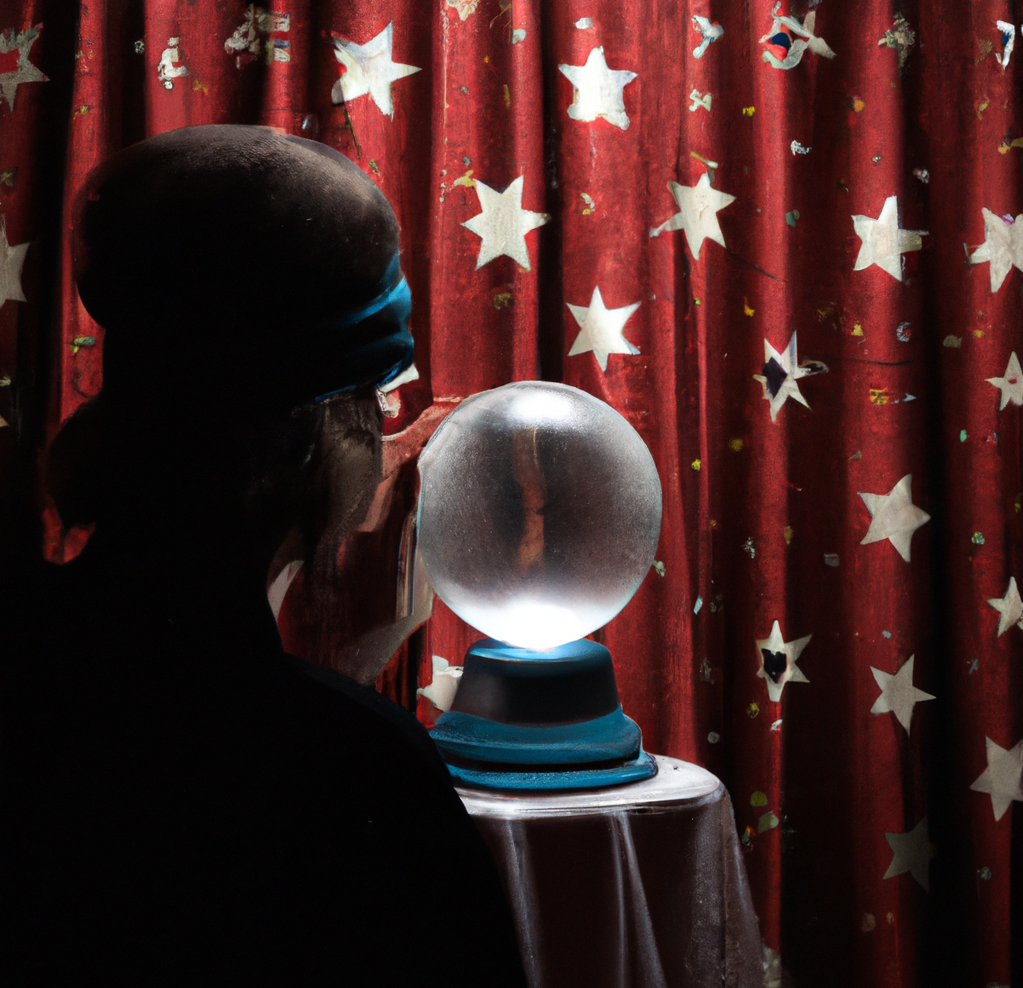
\includegraphics[height=6cm]{resources/medium.png}}
\caption{Picture of a medium generated by DALL·E 2}
\end{figure}

Let's say that we are very worried about a loved one who is at the other end of
the world, potentially doing dangerous activities. In order to get reassured, we
go and see a medium which would help us see our loved one and make sure he/she
is doing OK. The medium welcomes us with a cryptic sentence "Your friend is
eating your lunch". At this point, you remember that you forgot the lunch you
just on the counter of the kitchen, with your dog (Milly). It seems like the
medium has a \emph{non local} knowledge of the world: he knows something that
happened at a distance and this without communication with the remote event. But
then you realize that it's 11:30, you still have your lunch ticket peeking out
of your pocket, and you have Milly's hairs on your trousers. These three
elements are part of the \emph{context} of the current situation, and this is
probably how the medium guessed what happened (or rather what is happening). So
in the end the experience you just lived could be explained by a contextual
explanation of the event, and the medium has likely no non local abilities.

\section{Formal definition}
\label{sec:formal_definition}

After this wacky example of contextuality in our classical world, let's come back
on a quantum definition of if. First, some useful notions: The Pauli matrices are
$$X=\begin{pmatrix}
  0 & 1\\
  1 & 0
\end{pmatrix},Y=\begin{pmatrix}
  0 &  -i\\
  i & 0
\end{pmatrix} \text{ and } Z=\begin{pmatrix}
  1 & 0\\
  0 &-1
\end{pmatrix},$$
and we will also use the 2 by 2 identity matrix $I$.

We consider a thought experiment where we perform operations on a $n$ qubits
system, and I will show you that this thought experiment exhibits a contextual
behavior. The experiment is composed of several series of measurements using the
operators of the Pauli group. These operators are defined as a Pauli measurement
on each wire, with eventually a global phase. They are denoted
$$\mathcal{O} = s\bigotimes_{i=0}^n P_i$$
with $s\in\{\pm 1, \pm i\}$ and $P_i\in\{X,Y,Z,I\}$.
The result of such measurements is in $\pm 1$, and the overall result of the
experiment is the product of all measurement result. I will show you in Sec. 
\ref{sec:link_with_finite_geometries} that we can construct such experiments
where where quantum theory can produce a result non reproducible by classical,
non contextual theory.

\section{Link with other quantum specific properties}
\label{sec:link_with_other_quantum_specific_properties}

What we call quantum properties are quantum specific behaviors. They can arise
directly from the laws of quantum mechanics, such as the destructive nature of
measurements, but they can also be "meta" properties\footnote{this is not a
standard name in this context}, arising from the superposition of several other
quantum properties. Entanglement is the example of such a meta property
(we couldn't have entanglement without superposition), and contextuality is too:
the way quantum measurements work is absolutely necessary for quantum
contextuality (the fact that the measure projects the state on the space
corresponding to the result observed is the root of the contextual behaviors).

Understanding the links between these properties may help us build an intuition
concerning quantum computation. This is likely one of the reasons why they are
so studied! In that regard, let us have a look at one of the papers reveling on
of the deepest links in my opinion: the 2011 paper by S. Abramsky and A.
Brandenburger \cite{AB11}.

\section{Link with finite geometries}
\label{sec:link_with_finite_geometries}

As teased in Sec. \ref{sec:formal_definition}, this contextuality property can
be exhibited using measures on a $n$ qubits system. The corresponding thought
experiment is decomposed as such: on this $n$ qubits system, we will perform
several series of measurements. If we represent each operator used for a
measurement by a dot, and each series of measurement by a line, we obtain what we
call a finite geometry. 

This formalism can be complexified such that the finite geometry would live in a
vector space, and this allows us to perform interesting operations on those
geometries, but I will leave that as a teaser for an upcoming Medium article
(for more information, you may read \cite{dHG+22}).



\section{Link with quantum programs verification}
\label{sec:link_with_quantum_programs_verification}

\section*{At ColibrITD}

\bibliographystyle{alpha}
\bibliography{lib.bib}

\end{document}